\documentclass[12pt, a4paper]{article}
\usepackage{amsthm,amsfonts,amsmath,amssymb,amscd}
\usepackage[T2A]{fontenc}
\usepackage[utf8]{inputenc}
\usepackage[english, russian]{babel}
\usepackage{graphicx}
\usepackage{indentfirst}
\usepackage{cite}
\usepackage{psfrag}
\usepackage{yfonts}
\usepackage{titlesec}
\usepackage[center]{caption}
\newenvironment{compactlist}{
    \begin{list}{{$\bullet$}}{
      \setlength\partopsep{0pt}
      \setlength\parskip{0pt}
      \setlength\parsep{0pt}
      \setlength\topsep{0pt}
      \setlength\itemsep{0pt}
} }{
\end{list} }
\IfFileExists{pscyr.sty}{\usepackage{pscyr}}{}    %

\usepackage[top=2cm,bottom=2cm,left=2.5cm,right=1cm]{geometry}

\linespread{1.3}


\begin{document}
\begin{titlepage}
\begin{center}

\includegraphics[width=8cm, height=4cm]{MSU}
\end{center}
\begin{center}
Московский государственный университет имени М.В. Ломоносова\\
\vspace{0.1 cm}
Факультет вычислительной математики и кибернетики\\
\vspace{0.1 cm}
Магистерская программа <<Большие данные: инфраструктуры и методы решения задач>>

\vspace{3cm}
{\Large Черкашин Дмитрий Сергеевич }\\
\vspace{1cm}

{\bf\LARGE Параметризация звезд при полном отсутствии астрофизических параметров через их классификацию}\\ \vspace{2cm}
НАУЧНАЯ РАБОТА

\end{center}
\vspace{2cm}
\begin{flushright}

{\bf Научный руководитель:}\\
Научный сотрудник ИПИ РАН\\
Н.\,А. Скворцов

\end{flushright}

 \vspace{4.5cm}

\centerline {Москва, 2019}

\end{titlepage}
\newpage
\setcounter{page}{2}
\tableofcontents
\newpage

	\section{Введение}
	Одной из основных проблем астрофизики является изучение физических свойств, принадлежащих поверхностным слоям звезд. Параметры звезды (температура, гравитация, металличность и т.д.) могут быть получены из ее классификации на основе оптического, инфракрасного и ультрафиолетового спектра. Поскольку звезды наблюдаются сквозь межзвездную пыль, их свет тускнеет и краснеет, что затрудняет их параметризацию и классификацию. Этот эффект называется межзвездным поглощением - суммарный эффект рассеивания и истинного поглощения электромагнитного излучения пылью и газом. Знание межзвездного поглощения позволяет правильно интерпретировать наблюдательные данные и корректно оценивать параметры наблюдаемых объектов. Однако для получения параметров звезды и карты межзвездного поглощения нужно использовать большой телескоп или яркие объекты, чтобы получить спектральные распределения энергии с хорошим разрешением и достаточной точностью. Например, спектроскопические наблюдения с длительностью экспозиции 1 час на 2-метровом телескопе с низким (R $\sim$ 1000) и высоким (R $\sim$ 100 000) разрешением позволяют это сделать. 8-метровый телескоп справляется еще лучше. Такая работа была выполнена различными авторами, и был создан ряд эмпирических атласов (Straizys и Sviderskiene [1], Глушнева и др. [2], Алексеева и др. [3], Алексеева и др. [4], Pickles [5], Баньуло и др. [6], Ле Боргн и др. [7], Вальдес и др. [8], Хип и Линдлер [9], Фалькон-Баррозу и др. [10], Ву и др. [11]). Однако при сравнении данных для звезд, включенных в несколько атласов, обнаруживается большое количество расхождений [12].

	Другим способом построения карты межзвездного поглощения является ее оценка (а также оценка звездных параметров) по эволюционным трекам. Соответствующие процедуры были разработаны в работах Сичевского и Малкова [13], и применены к данным LAMOST. Однако знание звездных атмосферных параметров крайне желательно для применения этих процедур, ограничивая количество звезд, доступных для такой параметризации.

	Поэтому решение проблемы параметризации звезд на основе их фотометрии является актуальной проблемой [17]. Большое разнообразие фотометрических систем (см., Например, Straižys [18]) и недавно построенные большие фотометрические обзоры неба (такие как SDSS [19] и GALEX [20]), а также VO-инструменты для перекрестного отожествления объектов  создают возможность получения многоцветных фотометрических данных для миллионов объектов. Следовательно, это позволяет параметризировать объекты и определять межзвездное поглощение в Галактике. Однако для данной параметризации необходимы большие вычислительные мощности, которые проще всего получить, используя распределенные алгоритмы.

	Сравнительный анализ имеющихся трехмерных карт межзвездного поглощения был сделан Килпио и Малковым [21], и были найдены противоречивые результаты.

	Ранние пылевые карты использовали корреляцию между плотностью пылевого столба и распределением нейтрального водорода [25]. Эти данные были вытеснены картами пыли, предоставленными Schlegel et al. [26], который использовал микроволновые данные в полном небе, предоставленные миссией IRAS (инфракрасный астрономический спутник) и инструментом DIRBE (диффузный инфракрасный фоновый эксперимент) в миссии COBE (Космический Исследователь Фонов). При отображении плотности пылевого столба с помощью откалиброванной температуры пыли карты поглощения, предполагающие стандартный закон поглощения, оказались как минимум в два раза точнее, чем карты Бурштейна и Хейлса [25]. Преимущество этого метода заключается в том, что он не опирается на предварительно определенную модель звездного распределения. Однако данные карты по-прежнему неидеальны, из-за чего получение карты межзвездного поглощения во время решения задачи параметризации звезд позволит провести дополнительное сравнение.

	Успешная реализация европейской астрометрической космической миссии Gaia (вторая версия каталога миссий, Gaia DR2, была опубликована в апреле 2018 года [27]) позволяет решить ряд проблем звездной астрономии, таких как определение массы звезды, оценка возраста и другие. В частности, стало возможным улучшить результаты параметризации звезд, проведенной методом многоцветной фотометрии.

	Таким образом, проблема параметризации звезд на основе их фотометрии является актуальной на момент написания данной работы.
	\section{Родственные работы}
	\subsection*{Обратные задачи в астрофизике}
	\addcontentsline{toc}{subsection}{Обратные задачи в астрофизике}
	\subsubsection*{Теория}
	Астрофизика - по большей части наблюдательная наука, т.к. при изучении объекта обычно нет возможности на него воздействовать. Создание модели исследуемого объекта ученые-астрофизики осуществляют на основе анализа косвенной информации, которая поступает из космоса в виде различных излучений: эми, нейтронное, корпускулярное, гравитационно-волновое. Характеристики этих излучений являются следствием процессов, природу которых должен объяснить астрофизик. Хотя иногда ученые могут воздействовать на изучаемый объект (например, изучение поверхности планеты с помощью активных космических аппаратов), в большинстве случаев приходится по следствиям процессов, протекабщих на небесных телах, судить о причинах, их породивших, т.е. решать обратные задачи.

	В отличие от прямой задачи, решение которой связано с нахождением следствия некоторого процесса по известной исследователю причине, решения обратных задач связаны с тем, что один и тот же эффект может быть порожден разными причинами, например, из того факта, что вода кипит, вовсе не следует, что она нагрета до температуры 100ºC, поскольку вода может кипеть и при комнатной температуре, но при достаточно низком атмосферном давлении, т.е. кипение обуславливается либо высокой температурой, либо низким давлением.

	В математике хорошо известно, что подавляющее большинство обратных задач являются некорректно поставленными – малым возмущением исходных данных (данных наблюдений) могут соответствовать сколь угодно большие возмущения решения. Задача называется корректной, если:
	\begin{compactlist}
	\item ее решение существует
	\item решение единственно
	\item решение непрерывно зависит от входных данных
	\end{compactlist}

	иначе задача считается некорректной. Наиболее часто в случае обратных задач нарушается третье условие, то есть условие устойчивости решения. В этом случае возникает парадоксальная ситуация: несмотря на то, что задача математически сформулирована, ее решение невозможно получить обычными методами, из-за чего возникает ощущение, что некорректные задачи не имеют практического смысла. Однако по существу все задачи обработки и интерпретации результатов астрономических наблюдений, как и многих физических экспериментов, являются обратными и некорректно поставленными. До появления современных научно обоснованных методов исследователь, либо используя детальную физическую модель изучаемого явления сводил обратную задачу к нахождению небольшого числа параметров (что приводит к большим остаточным уклонениям наблюдательных данных от теоретических предсказаний), либо основываясь на физической интуиции отбирал из множества допустимых решений то, которое лучше всего соответствует здравому смыслу (выбор решения субъективен, что не характерно для научного метода исследований).
	
	Математически под обратной задачей понимается задача отыскания функции z(s) по функции u(x), получаемой из эксперимента или наблюдений и определяемой уравнением вида
	$$
	u(x)=A(x,z(s))
	$$
	где $A$ – некоторый оператор, устанавливающий причинно-следственную связь между $z(s)$ и $u(x)$. В уравнении по наблюдаемым следствиям процесса $u(x)$ нужно судить о причинах $z(s)$, породивших его.
	Во многих случаях обратная задача может быть представлена интегральным уравнением Фредгольдма 1-го рода
	$$
	u(x) = \int^a_b K(x, s)z(s) ds
	$$
	где $K(x, s)$ – ядро (непрерывное или квадратично суммируемое по переменным $x$, $s$), которое описывает конкретную модель исследуемого процесса.
	
	Математические трудности решения обратных задач связаны с тем, что обратный оператор $A^{-1}$ не является непрерывным. Поэтому если данные наблюдений $u(x)$ получены с некоторой ошибкой $\delta$($\delta u(x)$), то соответствующее приближенное решение, полученное стандартным методом,
	$$
	z\delta(s)= A -1 (u\delta(x))
	$$
	будет сколь угодно сильно отклоняться от решения, соответствующего идеально точным входным данным $u(x)$.
	
	Предлагаемые ранее методы решения обратных некорректных задач основывались прежде всего на интуиции авторов, и, хотя в ряде обратных задач удавалось получить важную физическую информацию, необходимость в строгой математической постановке и разработке численных методов решения этого важнейшего для современного естествознания круга проблем назрела к 60-м годам, особенно в связи с широким внедрением компьютеров в практику научных исследований.

	Предложенный российским академиком А.Н. Тихоновым метод решения некорректно поставленных задач состоит в том, что такие задачи рассматриваются как физически недоопределенные. Они <<плохо>> поставлены, множества их приближенных решений очень широки, даже неограниченны. Поэтому некорректные задачи нужно доопределить. Для этого необходима дополнительная (априорная) информация об искомом решении $z(s)$, вытекающая из обширного опыта всесторонних исследований данного процесса. Эта дополнительная информация об искомом решении должна быть известна заранее, до решения соответствующей некорректной задачи. Априорная информация позволяет сформулировать критерий отбора приближенного решения из множества приближенных решений уравнения и построить регуляризирующий алгоритм.

	Такой информацией могут служить сведения о гладкости искомого решения $z(s)$, его монотонности, выпуклости, неотрицательности, принадлежности к конечно-параметрическому семейству и т. п.

	Далее разберем типичный пример применения регуляризации к обратной задаче астрофизики.
	\subsubsection*{Анализ дифракционных кривых блеска, наблюдаемых при покрытии звезд Луной}
	При наблюдейнии звездных тел необходимо достигноуть как можно более высокого углового разрешения(минимальное угловое расстояние, на котором должны находиться два объекта для того, что бы их можно было различить в телескоп раздельно). Что бы этого добиться, телескопы запускаются в космос (угловое разрешение больше, чем при изучении тел на поверхности Земли через атмосферу), создают телескопы с линзами экстремально большого диаметра. Однако оказалось, что высокое угловое разрешение можно получить гораздо более простым и дешевым способом, наблюдая с поверхности Земли при помощи телескопа небольшого диаметра($\approx$ 1м) покрытия звезд Луной. Процесс затемнения диска звезды Луной будет иметь достаточную продолжительность для его получения кривой затмения звезды луной, которая будет обусловлена как геометрическим затмением, так и эффектами дифракции света звезды на краю диска Луны. Чем меньше будет угловой диаметр затмеваемой звезды, тем меньше будет высота дифракционных максимумов и тем ближе кривая блеска при покрытии звезды луной будет напоминать кривую геометрического затмения. Т.о., решая обратную задачу интерпретации кривой покрытия звезды Луной, можно определить угловой диаметр звезды и даже пытаться получать информацию о распределении яркости по диску звезды или о наличии околозвездной структуры(например, протопланетного диска вокруг звезды, ее близкого спутника и т.п. Т.к. и звезда, и наблюдаемый объект находятся за пределами неспокойной земной атмосферы, то атмосферные искажения не могут существенно повлиять на вид дифракционной кривой покрытия звезды Луной.  
	
	Математически рассматриваемая задача заключается в решении интегрального уравнения Фредгольма 1-го рода
	$$
	S(x)=\int^{\infty}_{-\infty} K(x-\chi)B(\chi) d\chi
	$$
	где $S(x)$ – наблюдаемая дифракционная картина изменения интенсивности при покрытии звезды Луной, $x(t)=V(t-t_0)$, $V$ – проекция линейной скорости движения Лунного края на его нормаль в направлении на проекцию звезды, $t$ – время, $t_0$ – момент времени, когда центр звезды точно проектируется на край лунного диска, $B(\chi)$ – искомая функция, выражающая стрип-распределение яркости по диску звезды (распределение, проинтегрированное вдоль прямых, параллельных лунному краю). Ядро $K(x-\chi)$ представляет собой дифракционную картину точечного источника, полученную с учетом влияния различных искажающих факторов.
	
	Естественной априорной информацией об искомой функции является ее монотонность или выпуклость, а также неотрицательность. Кроме того, в случае звезды с тонкой атмосферой, можно использовать аналитическое конечно-параметрическое представление функции $B(\chi)$ , полученное из теории. В случае, когда наблюдается покрытие двойной звезды или звезды, обладающей околозвездной структурой (аккреционный диск, планетная система), можно использовать регуляризирующий алгоритм Тихонова на множестве гладких неотрицательных функций

	Применение метода наблюдений покрытий звезд Луной к исследованию молодых звезд типа $Т$ Тельца позволило выявить внутренние части околозвездного (возможно, протопланетного) диска вокруг звезды DG в созвездии Тельца с угловым разрешением до $0,0001"$
	
	К настоящему времени методом лунных покрытий определены угловые диаметры сотен звезд, открыты тысячи новых тесных двойных звезд, изучена структура протопланетных дисков вокруг ряда молодых звезд. Т.о., при помощи регуляризации метод лунных покрытий превратился в мощный метод исследования звезд с очень высоким угловым разрешением.
	\subsection*{Методы минимизации функции нескольких переменных}
	\addcontentsline{toc}{subsection}{Методы минимизации функции нескольких переменных}
	При параметризации звезд потребуется минимизировать функцию нескольких параметров. Рассмотрим возможные методы минимизации.
	\subsubsection*{Метод градиентного спуска}
	Метод градиента в чистом виде формирует шаг по переменным как функцию от градиента $F(x)$ В текущей точке поиска. Простейший алгоритм поиска $\min F(x)$ записывается в векторной форме следующим образом:
	$$
	x^{i+1} = x^i - h * \nabla f(x^i)
	$$
	В скалярном виде:
	$$
	x^{i+1}_j = x^i_j - h * \frac{df}{dx^i_j}, j = 1,...,n
	$$
	Величина рабочего шага в направлении градиента зависит от величины градиента, котороую заранее учесть трудно, и от коэффициента пропорциональности шага, с помощью которого можно управльять эффективностью метода.
	Поиска каждой новой точки состоит из двух этапов:
	\begin{compactlist}
		\item Оценка градиента $F(x)$ путем вычисления частных производных от $F(x)$ по каждой переменной $x_j$
		\item Рабочий шаг по всем переменным одновременно
	\end{compactlist}
	Величина h сильно влияет на эффективность метода. Большей эффективностью обладает вариант метода, когда шаг по каждой переменной определяется направляющими косинусами градиента:
	$$
	x^{i+1}_j = x^i_j - h * \cos(\phi_j) = x^i_j - h * \frac{df/dx^i_j}{|\nabla f(x^i)|}
	$$
	Тогда величина рабочего шага не зависит от величины модуля градиента, и ею легче управлять изменением $h$. Шаг $h$ следует выбирать меньше 0.01, иначе метод расходится (метод может расходится и при таком шаге в зависимости от исследуемой функции).
	Но даже для хорошо обусловленных функций проблема выбора шага нетривиальна в силу отсутствия априорной информации о минимизируемой функции. Если шаг выбирается малым (чтобы гарантировать сходимость), то метод сходится медленно. Увеличение же шага (с целью ускорения сходимости) может привести к расходимости метода. Эту проблему решают алгоритмы с коррекцией (дроблением) шага:
	\begin{compactlist}
		\item $h^i = const = h$ (без коррекции)
		\item $h^i = 
				\left\{\begin{aligned}
				& \frac{h^{i-1}}{2},  f(x^i) < f(x^{i-1}) \\ 
				& h^{i-1},  f(x^i) > f(x^{i-1})
				\end{aligned}\right.$
		\item $h^i = 
				\left\{\begin{aligned}
				& h^{i-1},  \alpha_1 \le \alpha \le \alpha_2 \\ 
				& 2h^{i-1},  \alpha_1 > \alpha \\
				& \frac{h^{i-1}}{3},  \alpha_2 < \alpha
				\end{aligned}\right.$
	\end{compactlist}
	где $\alpha$ -  угол между градиентами на предыдущем и текущем шаге; $\alpha_1$ и $\alpha_2$ – заданные пороговые значения, выбираются субъективно (например, $\alpha_1$=$\pi$/6, $\alpha_2$=$\pi$/3).
		Вдали от оптимума направление градиента меняется мало, поэтому шаг можно увеличить (второе выражение), вблизи от оптимума направление резко меняется (угол между градиентами $f(x)$ большой), поэтому $h$ сокращается (третье выражение).
	
	Для оценки частных производных используются разностные методы:
	\begin{compactlist}
		\item Алгоритм с центральной пробой: $\frac{df}{dx_i} \approx 
		\frac{f(x_1,...,x_i+g_i,...,x_n)-f(x_1,...,x_i,...,x_n)}{g_i}$	
		\item Алгоритм с парными пробами: $\frac{df}{dx_i} \approx 
		\frac{f(x_1,...,x_i+g_i,...,x_n)-f(x_1,...,x_i-g_i,...,x_n)}{g_i}$	
	\end{compactlist}
	Где $g_i$ – пробный шаг по $i$-й переменной, выбираемый достаточно малым для разностной оценки производной.
	Первый вариант требует меньших затрат по сравнению со вторым (обычно затраты выражаются количеством вычислений критерия оптимальности), но позволяет получить решение менее точно, чем второй, и эта погрешность зависит от величины проб­ного шага.
	Условием окончания поиска может являться малость модуля градиента $F(X)$.
	
	Основным недостатком градиентного метода является необходимость частого вычисления производных от функции F(х). Этого недостатка лишен метод наискорейшего спуска.
	
	\subsubsection*{Метод наискорейшего спуска}
	В текущей точке вычисляется  $\nabla f(x)$, и затем в направлении градиента ищется $\min f(x)$. Практически это может быть осуществлено любым методом одномерной оптимизации (поиск по одному направлению – направление градиента), наиболее часто используется сканирование до первого локального минимума по направлению $\nabla f(x)$. В результате вдали от оптимума эффективность метода повышается, мы быстрее попадем в район оптимума, в окрестности которого эффективность метода снижается из-за частой смены направления поиска и приближается к эффективности метода градиента. В ряде случаев используют уменьшение шага поиска оптимума по направлению после каждой смены направления. Условием окончания поиска в этом случае является достижение заданной малой величины шага.
	
% #правки: объединить две статьи в один обзор
%Во-первых, недостаточно написать названия работ и их аннотации. Нужен их анализ, что там есть, каковы подходы, каковы недостатки с точки зрения настоящего исследования, что из этого есть смысл использовать в настоящем исследовании.
%Во-вторых, это не совсем родственные работы, это состояние работы на сегодня. Это, конечно, тоже нужно в этом разделе.
%А в качестве родственных можно описать подходы к решению обратных задач, подходы к их оптимизации, подходы к распределению обработки астрономических данных.
	\subsection*{Interstellar extinction from photometric surveys: application to four high-latitude areas. [29]}
	\addcontentsline{toc}{subsection}{Interstellar extinction from photometric surveys}
	В данной работе представлены различные аспекты и экспериментальные результаты параметризации звезд по многоцветной фотометрии, обсуждается построение трехмерной карты галактического межзвездного поглощения.

	Было показано, что с помощью достаточно качественной фотометрии можно рассчитать трехмерную карту поглощения, сравнив каталогизированную многоцветную фотометрию с фотометрией, полученной из уравнения модуля расстояний, закона межзвездного поглощения и расстояния. Отсутствие самосогласованной фотометрии для звезд, перечисленных в одном обзоре, ранее препятствовало такому определению, но это стало возможным в современных крупных многоцветных обзорах и в эпоху Виртуальной обсерватории.

	С появлением крупных, существующих и будущих фотометрических съемок и развитием вычислительной мощности и методов анализа данных (в частности, VO-инструментов для перекрестного отожествления), поглощение теперь может быть вычислено для миллионов звезд в разумных пределах времени.

	\subsection*{Verification of photometric parallaxes with Gaia DR2 data. [30]}
	\addcontentsline{toc}{subsection}{Verification of photometric parallaxes with Gaia DR2 data}
	В этой статье описывается проверка метода, проанализированного в [29] с использованием данных Gaia DR2, обсуждается, как включение параллаксов Gaia в процедуру повышает точность параметризации, и как выбирать / обрабатывать объекты с неизвестным параллаксом Gaia для параметризации.

	Было показано, что параметризация звезд ближе 4400 pc является успешной при условии правильного определения класса светимости, представляется целесообразным включить в процедуру параметризации информацию о фотометрии не МС-звезд (суб-карликов, гигантов и супергигантов), взятую из литературы или определенную собственными усилиями.
	\section{Постановка}
	\subsection*{Цель}
	\addcontentsline{toc}{subsection}{Цель}
	Разработка методов и средств распределенного анализа данных в в области звездной астрономии и астрофизике.
	\subsection*{Задачи}
	\addcontentsline{toc}{subsection}{Задачи}
	\begin{compactlist}
		\item Разработка концептуального представления данных о фотометрических спектрах звёзд и отображение в него схем оригинальных каталогов для трансформации данных множественных наблюдений звёзд в общее представление.
		\item Разработка подхода к организации доступа и разрешению сущностей (перекрёстному отождествлению) среди множественных наблюдений звёзд в неоднородных данных обзоров неба.
		\item Модификация алгоритма параметризации звезд на основе методов решения обратных задач
		\item Разработка параллельной распределённой реализации предложенных подходов
	\end{compactlist}
	\section{Описание и загрузка используемых каталогов звездного неба}
В рамках курсовой взяты отдельные каталоги из множества потенциально применимых при решении данной задачи, и небольшой участок звездного неба, сектор с центром в созвездии Гидра радиусом $5^{\circ}$. Для возможности распределенной обработки каталоги необходимо загрузить в hdfs.
	\subsection*{AllWISE Data Release}
	\addcontentsline{toc}{subsection}{AllWISE Data Release}
	Wide-field Infrared Survey Explorer - это миссия NASA Medium Class Explorer, которая провела цифровую съемку всего неба в середине 3.4, 4.6, 12 и 22 полосы пропускания (далее W1, W2, W3 и W4). Программа AllWISE расширяет работу успешной миссии Wide-field Infrared Survey Explorer, объединяя данные с этапов криогенной и посткриогенной съемки, чтобы сформировать наиболее полное представление о среднем инфракрасном небе, доступном в настоящее время. AllWISE выпустил новый каталог источников и атлас изображений с повышенной чувствительностью и точностью по сравнению с более ранними выпусками данных WISE. Усовершенствованная обработка данных для AllWISE использует два полных покрытия неба для измерения движений источника для каждого источника каталога и для создания обширной базы данных для этих объектов.
	\newline
	\begin{table}[h]
	\centering
	\begin{tabular}{|l|l|}
	\hline
	Атрибут & Описание \\ \hline
	AllWISE & WISE Название каталога релизов All-Sky \\ \hline
	DEJ2000 & Склонение (J2000) \\ \hline
	RAJ2000 & Прямое восхождение (J2000) \\ \hline
	Hmag & Величина в диапазоне H (1,65 мкм) \\ \hline
	e\underline{ }Hmag & Погрешность по величине H \\ \hline
	Jmag & Величина в диапазоне J (1,25 мкм) \\ \hline
	e\underline{ }Jmag & Погрешность по величине J \\ \hline
	Kmag & Величина в диапазоне K (2.17 мкм) \\ \hline
	e\underline{ }Kmag & Погрешность по величине Ks \\ \hline
	W1mag & Величина в диапазоне W1 (3,35 мкм) \\ \hline
	e\underline{ }W1mag & Погрешность по величине W2 \\ \hline
	W2mag & Величина в диапазоне W2 (4.6 мкм) \\ \hline
	e\underline{ }W2mag & Погрешность по величине W2 \\ \hline
	W3mag & Величина в диапазоне W3 (11,6 мкм) \\ \hline
	e\underline{ }W3mag & Погрешность по величине W3 \\ \hline
	W4mag & Величина в диапазоне W4 (22,1 мкм) \\ \hline
	e\underline{ }W4mag & Погрешность по величине W4 \\ \hline	\end{tabular}
	\caption{Список атрибутов каталога}
	\end{table}
	\subsection*{DENIS Data Release of the Southern Sky}
	\addcontentsline{toc}{subsection}{DENIS Data Release of the Southern Sky}
	Этот каталог является последней инкрементной версией проекта DENIS. Он состоит из набора 355,220,325 точечных источников, обнаруженных при обследовании DENIS в 3662 полосах (охватывающих каждые 30 градусов по склонению и 12 угловых минут при прямом восхождении). Данные в этом выпуске охватывают приблизительно 16700 квадратных градусов южного неба. Положение общего извлеченного точечного источника обеспечивается точность лучше 1 арксек, а его величина лучше 0,1 мкс. Ученые и инженеры из семи европейских стран и из Бразилии участвуют в оценке и анализе данных.
	\newline
	\begin{table}[h]
	\centering
	\begin{tabular}{|l|l|}
	\hline
	Атрибут & Описание \\ \hline
	DENIS & DENIS идентификатор \\ \hline
	DEJ2000 & Склонение (J2000) \\ \hline
	RAJ2000 & Прямое восхождение (J2000) \\ \hline
	Imag & Величина в диапазоне I (0,83 мкм)\\ \hline
	e\underline{ }Imag & Погрешность величины в диапазоне I\\ \hline
	Jmag & Величина в диапазоне J (1,25 мкм) \\ \hline
	e\underline{ }Jmag & Погрешность величины в диапазоне J\\ \hline
	Kmag & Величина в диапазоне K (2.17 мкм)\\ \hline
	e\underline{ }Kmag & Погрешность величины в диапазоне K\\ \hline
	\end{tabular}
	\caption{Список атрибутов каталога DENIS}
	\end{table}
	\subsection*{Загрузка каталогов звездного неба}
	\addcontentsline{toc}{subsection}{Загрузка каталогов звездного неба}
	Для загрузки, а так же для последующих вычислений, был использован фреймворк Apache Spark версии 2.4.0.cloudera2 через Scala версии 2.11.12. Данные были загружены через API с сайта http://vizier.u-strasbg.fr при помощи пакета org.apache.http, после чего загружалить на hdfs в формате ORC.

	В результате было загружено 135.677 звезд из каталога DENIS и 1.169.013 звезд из каталога ALLWISE.
	
	Выбранная для хранения схема:
	\newline
	\begin{figure}[h]
	\centering
	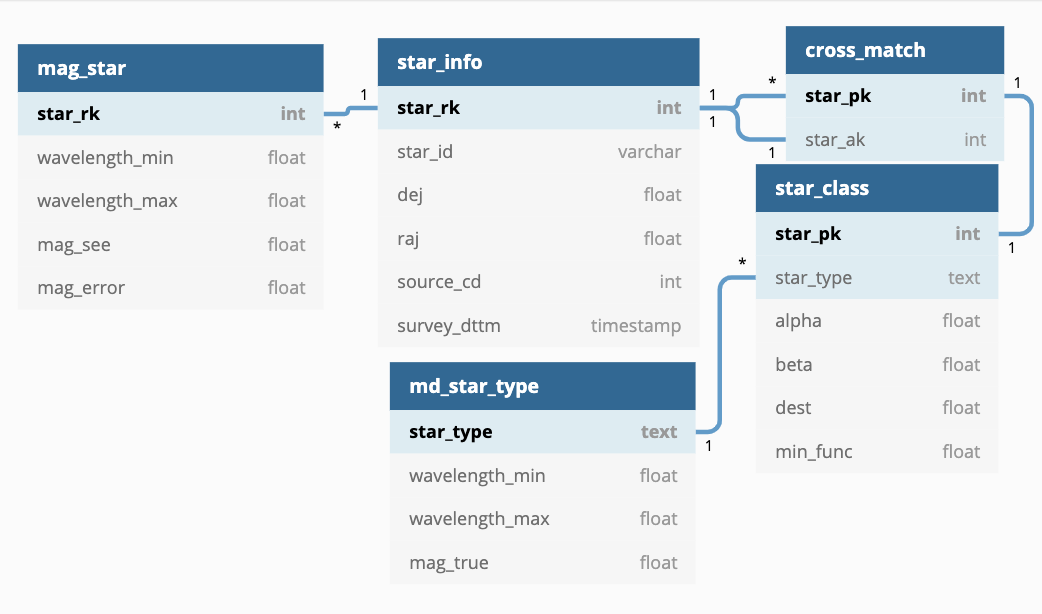
\includegraphics[width=15cm]{dds.png}
	\caption{Гистограмма расстояния между координатами в ALLWISE и DENIS}
	\end{figure}
	\begin{compactlist}
		\item $star\_info$ - Основная информация о звезде: сгенерированный ключ, ключ в источнике, координаты, код источника, дата создания обзора
		\item $mag\_star$ - Видимый спектр звезды: сгенерированный ключ, рассматриваемый интервал длины волны, блеск для данного интервала, ошибка блеска для данного интервала
		\item $cross\_match$ - Результат кросс-отожествления каталогов: родительский ключ звезды, дочерний ключ звезды
		\item $md\_star\_type$ - Справочная информация о типах звезд: рассматриваемый интервал длины волны, блеск для данного интервала
		\item $star\_class$ - Результат параметризации звезд: сгенерированный ключ, тип звезды, параметры $\alpha, \beta, d$, значение функционала (см. реализацию алгоритма параметризации)
	\end{compactlist}

	\section{Кросс-отожествление каталогов обзоров звездного неба}
	\subsection*{Проблемы, способы решения}
	\addcontentsline{toc}{subsection}{Проблемы, способы решения}
	Задача кросс-отождествления объектов в разных каталогах состоит в поиске проявлений одного и того же источника в двух или более списках координат. При этом приходится иметь дело со следующими проблемами:
	\begin{compactlist}
		\item плохая координатная точность, разные системы координат каталогов, разные эпохи наблюдений (для случаев большого собственного движения), что приводит к тому, что координаты одного и того же объекта в разных списках в общем случае не совпадают либо систематически, либо случайным образом;
		\item разные чувствительности и, следовательно, разные предельные величины в каталогах. В итоге объект может присутствовать только в одном из списков, а в более глубоких каталогах будут присутствовать объекты, которых нет в других списках.
	\end{compactlist}
	Для отождествления списков объектов могут применяться следующие способы:
	\begin{compactlist}
		\item {\itshape Структурный.} Выделяются некоторые характерные множества объектов — геометрические конфигурации, и сопоставляются такие конфигурации из разных списков. Основная область применения этого метода — первичная астрометрическая привязка при наблюдениях, сопоставление звезд с кадра (координаты на ПЗС-матрице) и из каталога (координаты на небе). Обычно используется метод треугольников (их углы или отношения сторон инвариантны относительно масштабирования и поворота), однако встречаются алгоритмы, работающие с более сложными конфигурациями.
		\item {\itshape Координатный.} Сопоставляются все объекты разных каталогов, имеющие взаимные расстояния меньше некоторого предела. Это самый простой и часто используемый на практике вариант. Проблемы возникают, если в рассматриваемой окрестности объекта (задаваемой, скажем, точностью определения координат или величиной ожидаемого собственного движения) оказывается несколько объектов-кандидатов из другого каталога — получается неоднозначное сопоставление. Исправляется подбором предела. Есть возможность улучшения точности при помощи использования погрешности измерения координат.
		\item {\itshape Координатное сопоставление с фильтрацией объектов.} Основная идея заключается в использовании дополнительной информации об объектах и введении основанного на ней критерия, позволяющего выбрать из всех возможных кандидатов наиболее подходящий. Так, если в каталогах имеются измерения в близких спектральных диапазонах, то величины объекта в них будут совпадать (в границах соответствующих погрешностей). Если полосы каталогов существенно различны, можно использовать информацию об ожидаемых показателях цвета объектов — вычислять эти показатели всех пар-кандидатов и отбирать физически разумные либо совпадающие с основной массой показателей цвета всех получаемых пар в исследуемой площадке после фильтрации отскоков. Алгоритм можно улучшить, учитывая эпоху наблюдения - если звезда имеет собственное движение, перекрёстную идентификацию множества её наблюдений лучше проводить между ближайшими по времени наблюдениями.
	\end{compactlist}
	\subsection*{Реализация}
	\addcontentsline{toc}{subsection}{Реализация}
	В данной работе используется координатный метод, ввиду простоты его реализации, с планами добавления фильтрации объектов по спектральному диапазону. Для этого был использован пакет AstroML для Spark с пределом расстояния в 1 arcsec, в результате получил 112.531 успешных сопоставлений звезд. (формат на рис.1)

	Как видно из гистограммы, основное расстояние между координатами звезды в разных каталогах в пределах 0.5 arcsec.
	
	\begin{figure}[h]
	\centering
	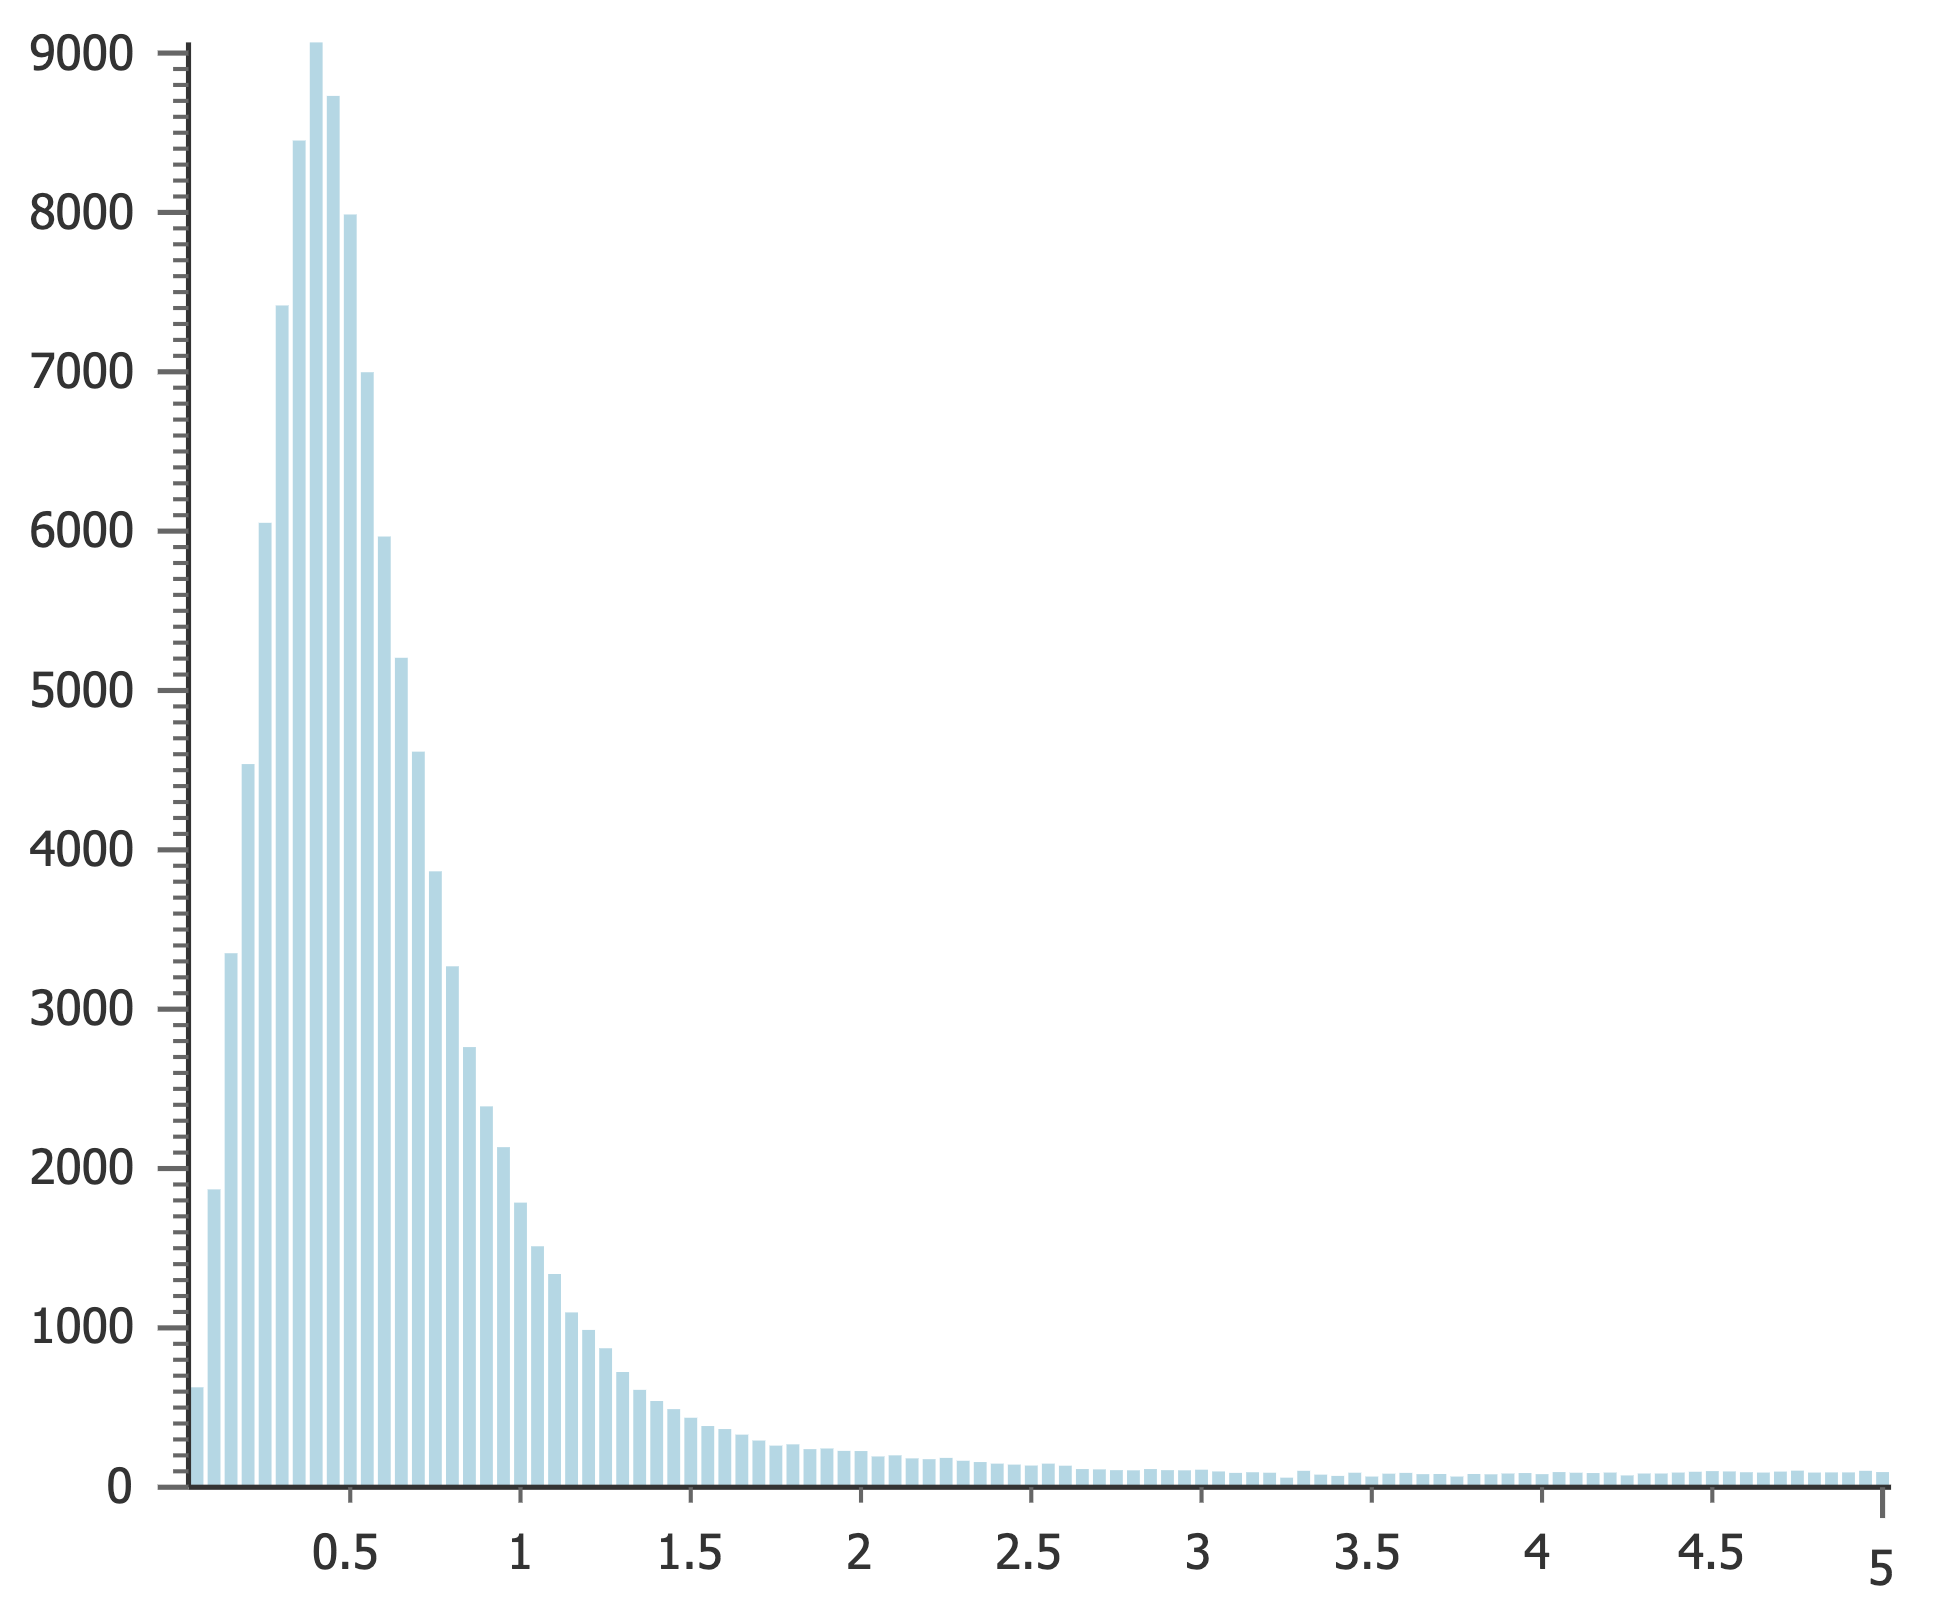
\includegraphics[width=7cm]{lol}
	\caption{Гистограмма расстояния между координатами в ALLWISE и DENIS}
	\end{figure}
	\section{Распределенный алгоритм параметризации звезд}
	\subsection*{Теория}
	\addcontentsline{toc}{subsection}{Алгоритм обратного спектрального анализа}
	Для нахождения спектрального типа $SpT$, расстояния до звезды $d$ и межзвездное поглощение $A_V$, необходимо минимизировать функционал
	$$
	D^2 = \sum_{i=1}^N \left(\frac{m_{obs,i}-m_{calc,i}}{\Delta m_{obs,i}} \right)^2
	$$
	где суммирование происходит по всем известным диапазонам ($N = 10$), и
	$$
	m_{calc,i} = M_i(SpT) + 5 \log d - 5 + A_i(A_V)
	$$
	где $m_{obs,i}$ и $m_{calc,i}$ -- видимая звездная величина (блеск) и ее погрешность наблюдения в i-той фотометрической полосе соответсвенно.

	$A_i(A_V) = k_i*A_V$ - закон межзвездного поглощения для i-той фотометрической полосы. Чем меньше длина волны, тем сильнее эффект межзвездного поглощения (см. Рис. 2). Для того, что бы это учитывать, существует $k_i$ - коэффициент затухания блеска для i-той фотометрической полосы. Такие расчеты поглощения для классических и современных фотометрических систем были сделаны, например, в работах Heiser (1977), Rieke and Lebofsky (1985), Schlegel et al. (1998), Draine (2003), Wright et al. (2010), Schlafly and Finkbeiner (2011), Yuan et al. (2012)[31].
	\begin{figure}[h]
	\centering
	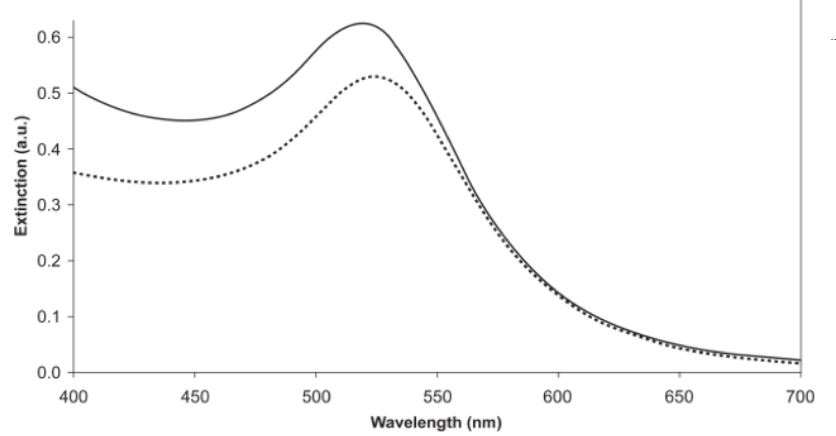
\includegraphics[width=11cm]{extinction}
	\caption{Абсолютный спектр звезды (непрерывная линия) \newline и ее видимый спектр (пунктирная линия)}
	\end{figure}

	Мы воспользуемся последним источником (см Таблица 3).
	\begin{table}[!ht]
	\centering
	\setlength{\tabcolsep}{3pt}
	\begin{tabular}{|l|l|l|l|l|l|l|l|}
	\hline
	Длина волны & I & J & K & W1 & W2 & W3 & W4 \\ \hline
	Коэффициент & 1.71 & 0.72 & 0.30 & 0.18 & 0.16 & 0.14 & 0.11 \\ \hline
	\end{tabular}
	\caption{Коэффициенты межзвездного поглощения}
	\end{table}

	$M_i(SpT)$ - абсолютный блеск в i-той фотометрической полосе. Необходимы абсолютные величины звезд разных спектральных типов в соответствующих фотометрических системах. Такие данные для различных исследований можно найти, например, в Covey et al. (2007), Kraus и Hillenbrand (2007), Findeisen и Hillenbrand (2010), Findeisen et al. (2011), Pecaut and Mamajek (2013)). Данные для M-звезд также можно найти в Bochanski et al. (2007) и West et al. (2011).
	\newline
	\begin{table}
	\centering
	\small
	\setlength{\tabcolsep}{3pt}
	\begin{tabular}{|l|l|l|l|l|l|l|l|l|l|}
	\hline
	SpT & MB    & MR    & MI    & MJ    & MK    & MW1   & MW2   & MW3   & MW4   \\ \hline
	B8  & 0.32  & 0.39  & 0.04  & 0.34  & 0.62  & 0.01  & 0.10  & 0.11  & 1.00  \\ \hline
	A0  & 1.58  & 0.47  & 0.72  & 1.04  & 1.28  & 0.54  & 0.58  & 0.56  & 0.30  \\ \hline
	A2  & 2.41  & 1.22  & 1.39  & 1.65  & 1.87  & 1.12  & 1.15  & 1.12  & 1.10  \\ \hline
	A5  & 3.14  & 1.88  & 1.95  & 2.15  & 2.32  & 1.53  & 1.52  & 1.48  & 1.75  \\ \hline
	A7  & 3.47  & 2.21  & 2.23  & 2.40  & 2.55  & 1.75  & 1.71  & 1.66  & 2.08  \\ \hline
	F0  & 3.94  & 2.77  & 2.68  & 2.79  & 2.90  & 2.10  & 2.01  & 1.96  & 2.61  \\ \hline
	F2  & 4.23  & 3.10  & 2.96  & 3.04  & 3.13  & 2.32  & 2.20  & 2.14  & 2.89  \\ \hline
	F5  & 5.01  & 3.90  & 3.68  & 3.69  & 3.74  & 2.85  & 2.67  & 2.61  & 3.61  \\ \hline
	..  & ..    & ..    & ..    & ..    & ..    & ..    & ..    & ..    & ..    \\ \hline
	\end{tabular}
	\caption{Абсолютные значения видимой звездной величины при различных спектральных типах звезд}
	\end{table}
	$A_V$ - коэффициент преломления для звезды, находящейся на расстоянии $d$, вычисляется по формуле:
	$$
	A_V(d, b) = \frac{a_O \beta}{\sin |b|} \left( 1 - e^{\frac{-d \sin |b|}{\beta}}\right)
	$$
	$a_O$ - коэффициент поглощения (параметр),
	$\beta$ - коэффициент вертикального поглощения преломляющегося света,
	$b$ - долгота

	\subsection*{Реализация}
	%#правки с экспериментами надо будет активно разбираться дальше, сейчас же, не весной. Перейти на наш кластер и развивать эксперименты
	\addcontentsline{toc}{subsection}{Реализация}
	Алгоритм реализован на Spark. Для каждой звезды ищем минимум функционала
	\begin{verbatim}
    pow(((col("Imag")  - (col("MI")  + lit(5) * log(col("b")) - lit(5) +
    col("I") * (col("a_0") * col("beta") * (lit(1) - exp((- col("b") *
    sin(abs(col("DEJ2000"))))))/sin(abs(col("DEJ2000"))))))/(col("e_Imag")))
    , lit(2))  +
    ...
    ...
    )
    \end{verbatim}
	Затем отбираем минимальный, репартиционируем, сохраняем
	\newline
	\begin{verbatim}
	res_0
	.groupBy(col("DENIS"), col("AllWISE"))
	.agg(min(col("functional")).as("functional"))
	.join(res_0, Seq("DENIS", "AllWISE", "functional"))
	.repartition(2000)
	.write.mode("overwrite").saveAsTable("user_dcherkashin.vkr_res");
	\end{verbatim}
	В результате получаем связку <<координаты -- класс звзеды -- расстояние до звезды -- коэффициент поглощения -- коэффициент вертикального поглощения преломляющегося света>>
	\begin{verbatim}
+----------+---------+---+--+----+----+
|   RAJ2000|  DEJ2000|SpT| b| a_0|beta|
+----------+---------+---+--+----+----+
|130.895126| 1.711113| B8|30|0.01|  30|
| 134.26753|-1.468054| B8|30|0.01| 270|
| 134.26753|-1.468054| B8|60|0.09|  30|
| 134.26753|-1.468054| B8|30|0.03|  90|
|134.859394| 2.091834| A5|30|0.06|  30|
|134.859394| 2.091834| A5|90|0.01| 180|
|134.859394| 2.091834| A5|30|0.03|  60|
|134.859394| 2.091834| A5|60|0.02|  90|
|136.378296| 1.129839| F0|30|0.06|  30|
|136.378296| 1.129839| F0|30|0.03|  60|
|..........|.........|...|..|....|....|
+----------+---------+---+--+----+----+
\end{verbatim}
\textbf{Результаты очень странные, скорее всего таблица абсолютных значений неверна, но оно слишком долго считается(какая-то дичь либо с репартиционированием, либо с форматом parquet, из-за чего огромный Shuffle Spill, и подсчет ведется только на 8 тачках из 1000 доступных) для того, что бы перепроверить это быстро}
	\section{Планы на будущее}
	%#правки Планы на будущее нужно будет поправить вместе в диалоге.
	\begin{compactlist}
		\item Добавить новые источники (Gaia DR2, IPHAS DR2, LAMOST)
		\item Реализовать фильтрацию звезд во время перекрестного отождествления
		\item Доработать алгоритм обратного спектрального анализа таким образом, что бы при минимизации функциоанала учитывались значения полученного коэффициента преломления для соседних звезд, воспользоваться другими подходами к оптимизации процедуры и точности определения параметров.
	\end{compactlist}



\newpage
\addcontentsline{toc}{section}{Список литературы}
\begin{thebibliography}{00}
\bibitem{1}
    \textit{Straizys, V.; Sviderskiene, Z.} Energy distribution in the stellar spectra of different spectral types and luminosities. Vilnius Astronomijos Observatorijos Biuletenis 1972, 35, 3.
\bibitem{2}
    \textit{Glushneva, I.N.; Kharitonov, A.V.; Kniazeva, L.N.; Shenavrin, V.I.} Secondary spectrophotometric standards. Astron. and Astrophys. Suppl. Ser 1992, 92, 1–29.
\bibitem{3}
    \textit{Alekseeva, G.A.; Arkharov, A.A.; Galkin, V.D.; Hagen-Thorn, E.I.; Nikanorova, I.N.; Novikov, V.V.; Novopashenny, V.B.; Pakhomov, V.P.; Ruban, E.V.; Shchegolev, D.E.} The Pulkovo Spectrophotometric Catalog of Bright Stars in the Range from 320 TO 1080 NM. Baltic Astronomy 1996, 5, 603–838.
\bibitem{4}
    \textit{Alekseeva, G.A.; Arkharov, A.A.; Galkin, V.D.; Hagen-Thorn, E.I.; Nikanorova, L.N.; Novikov, V.V.; Novopashenny, V.B.; Pakhomov, V.P.; Ruban, E.V.; Shechegolev, D.E.} The Pulkovo spectrophotometric catalog of bright stars in the range from 320 to 1080 NM - A supplement. Baltic Astronomy 1997, 6, 481–496. Pickles, A.J. A Stellar Spectral Flux Library: 1150-25000 A. Publ. Astron. Soc. Pac 1998, 110, 863–878. Bagnulo, S.; Jehin, E.; Ledoux, C.; Cabanac, R.; Melo, C.; Gilmozzi, R.; ESO Paranal Science Operations Team. The UVES Paranal Observatory Project: A Library of High- Resolution Spectra of Stars across the Hertzsprung-Russell Diagram. The Messenger 2003, 114, 10–14.
\bibitem{5}
    \textit{Le Borgne, J.F.; Bruzual, G.; Pello, R.; Lancon, A.; Rocca-Volmerange, B.; Sanahuja, B.; Schaerer, D.; Soubiran, C.; Vilchez-Gomez, R.} STELIB: A library of stellar spectra at R $\sim$ 2000. Astron. Astrophys 2003, 402, 433–442, [astro-ph/0302334].
\bibitem{6}
    \textit{Valdes, F.; Gupta, R.; Rose, J.A.; Singh, H.P.; Bell, D.J.} The Indo-US Library of Coude Feed Stellar Spectra. Astrophys. J. Suppl. Ser 2004, 152, 251–259, [astro-ph/0402435].
\bibitem{7}
    \textit{Heap, S.R.; Lindler, D.J.} Hubble’s Next Generation Spectral Library (NGSL). From Stars to Galaxies: Building the Pieces to Build Up the Universe; Vallenari, A.; Tantalo, R.; Portinari, L.; Moretti, A., Eds., 2007, Vol. 374, Astronomical Society of the Pacific Conference Series, p. 409.
\bibitem{8}
    \textit{Falcon-Barroso, J.; Sanchez-Blazquez, P.; Vazdekis, A.; Ricciardelli, E.; Cardiel, N.; Cenarro, A.J.; Gorgas, J.; Peletier, R.F.} An updated MILES stellar library and stellar population models. Astron. Astrophys 2011, 532, A95, [1107.2303].
\bibitem{9}
    \textit{Wu, Y.; Singh, H.P.; Prugniel, P.; Gupta, R.; Koleva, M.} Coude-feed stellar spectral library - atmospheric parameters. Astron. Astrophys 2011, 525, A71, [arXiv:astro-ph.SR/1009.1491].
\bibitem{10}
    \textit{Mironov, A.V.; Zakharov, A.I.; Moshkalev, V.G.; Malkov, O.Y.; Kilpio, E.Y.} On the construction of a new 3d atlas of stellar spectral energy distributions. Baltic Astronomy 2014, 23, 286–290.
\bibitem{11}
    \textit{Sichevsky, S.; Malkov, O.} Estimating stellar parameters and interstellar extinction from evolutionary tracks. Baltic Astronomy 2016, 25, 67–74.
\bibitem{12}
    \textit{Sichevskij, S.G.} Estimation of a star’s radius from its effective temperature and surface gravity taking into account stellar evolution. Astronomy Reports 2016, 60, 816–830.
\bibitem{13}
    \textit{Sichevskij, S.G.} Determining basic characteristics of stars from evolutionary computations. Astronomy Reports 2017, 61, 193–205.
\bibitem{14}
    \textit{Sichevskij, S.G.} Estimates of the radii, masses, and luminosities of LAMOST stars. Astrophysical Bulletin 2017, 72, 51–57.
\bibitem{15}
    \textit{Malkov, O.Y.} Interstellar Extinction from Large Surveys. Baltic Astronomy 2003, 12, 514–519.
\bibitem{16}
    \textit{Straizys, V.} Multicolor stellar photometry; 1992.
\bibitem{17}
	\textit{Malkov, O.Y.} Interstellar Extinction from Large Surveys. Baltic Astronomy 2003, 12, 514–519.
\bibitem{18}
	\textit{Straizys, V.} Multicolor stellar photometry; 1992.
\bibitem{19}
	\textit{Aihara, H.; Allende Prieto, C.; An, D.; Anderson, S.F.; Aubourg, E.; Balbinot, E.; Beers, T.C.; Berlind, A.A.; Bickerton, S.J.; Bizyaev, D.; Blanton, M.R.; Bochanski, J.J.; Bolton, A.S.; Bovy, J.; Brandt, W.N.; Brinkmann, J.; Brown, P.J.; Brownstein, J.R.; Busca, N.G.; Campbell, H.; Carr, M.A.; Chen, Y.; Chiappini, C.; Comparat, J.; Connolly, N.} The Eighth Data Release of the Sloan Digital Sky Survey: First Data from SDSS-III. Astrophys. J. Suppl. Ser 2011, 193, 29, [arXiv:astro-ph.IM/1101.1559].
\bibitem{20}
	\textit{Martin, D.C.; Fanson, J.; Schiminovich, D.; Morrissey, P.; Friedman, P.G.; Barlow, T.A.; Conrow, T.; Grange, R.; Jelinsky, P.N.; Milliard, B.; Siegmund, O.H.W.; Bianchi, L.; Byun, Y.I.; Donas, J.; Forster, K.; Heckman, T.M.; Lee, Y.W.; Madore, B.F.; Malina, R.F.; Neff, S.G.; Rich, R.M.; Small, T.; Surber, F.; Szalay, A.S.; Welsh, B.; Wyder, T.K.} The Galaxy Evolution Explorer: A Space Ultraviolet Survey Mission. Astrophys. J. Lett 2005, 619, L1–L6, [astro-ph/0411302].
\bibitem{21}
	\textit{Kilpio, E.Y.; Malkov, O.Y.} A study of interstellar absorption in the galaxy. Astronomy Reports 1997, 41, 10–18.
\bibitem{22}
	\textit{Kilpio, E.Y.; Malkov, O.Y.} Development of a synthetic model of interstellar extinction. Baltic Astronomy 1997, 6, 358.
\bibitem{23}
	\textit{Hakkila, J.; Myers, J.M.; Stidham, B.J.; Hartmann, D.H.} A Computerized Model of Large-Scale Visual Interstellar Extinction. Astron. J 1997, 114, 2043.
\bibitem{24}
	\textit{Malkov, O.; Kilpio, E.} A Synthetic Map of the Galactic Interstellar Extinction. Astrophys. Space. Sci 2002, 280, 115–118.
\bibitem{25}
	\textit{Burstein, D.; Heiles, C.} Reddenings derived from H I and galaxy counts - Accuracy and maps. Astron. J 1982, 87, 1165–1189.
\bibitem{26}
	\textit{Schlegel, D.J.; Finkbeiner, D.P.; Davis, M.} Maps of Dust Infrared Emission for Use in Estimation of Reddening and Cosmic Microwave Background Radiation Foregrounds. Astrophys. J 1998, 500, 525–553, [astro-ph/9710327].
\bibitem{27}
	\textit{Gaia Collaboration.; Brown, A.G.A.; Vallenari, A.; Prusti, T.; de Bruijne, J.H.J.; Babusiaux, C.; Bailer-Jones, C.A.L.; Biermann, M.; Evans, D.W.; Eyer, L.; } Gaia Data Release 2. Summary of the contents and survey properties. Astron. Astrophys 2018, 616, A1, [1804.09365].
\bibitem{28}
	\textit{Malkov, O.; Dluzhnevskaya, O.; Karpov, S.; Kilpio, E.; Kniazev, A.; Mironov, A.; Sichevskij, S.} Cross Catalogue Matching with Virtual Observatory and Parametrization of Stars. Baltic Astronomy 2012, 21, 319–330.
\bibitem{29}
	\textit{Malkov, O.; Karpov, S.; Kilpio, E.; Sichevsky, S.; Chulkov, D.; Dluzhnevskaya, O.; Kovaleva, D.; Kniazev, A.; Mickaelian, A.; Mironov, A.; Murthy, J.; Sytov, A.; Zhao, G.; Zhukov, A.} Interstellar extinction from photometric surveys: application to four high-latitude areas. Open Astronomy 2018, 27, 62–69.
\bibitem{30}
	\textit{Oleg Malkov, Sergey Karpov, Dana Kovaleva, Sergey Sichevsky, Dmitry Chulkov, Olga Dluzhnevskaya, Alexey Kniazev, Areg Mickaelian, Alexey Mironov, Jayant Murthy, Alexey Sytov, Gang Zhao and Aleksandr Zhukov} Verification of photometric parallaxes with Gaia DR2 data 2018
\bibitem{31}
	\textit{H. B. Yuan, X. W. Liu and M. S. Xiang} Empirical extinction coefficients for the GALEX, SDSS, 2MASS and WISE passbands, 2012
\end{thebibliography}
\end{document}